\documentclass{article}
\usepackage[margin=3cm]{geometry}
\usepackage{graphicx}
\usepackage{fancyvrb}

\title{Labwork 7: Stretch Image by Reduce}
\author{Le Nhu Chu Hiep}

\begin{document}
\maketitle

\section{Algorithm}

\subsection{Device Data}

Since cudaMalloc, cudaMemcpy and cudaFree are boring stuff, I write a struct to handle them.

\begin{Verbatim}[fontsize=\small]
template<typename T>
struct DeviceData {
    int size;
    T *data;
    const int threadSize = 512;
    int blockSize;

    DeviceData(T *data, int size) {
        this->size = size;
        const int realSize = sizeof(T) * this->size;
        cudaMalloc(&this->data, realSize);
        getLastCudaError("Could not allocate a DeviceData...");
        cudaMemcpy(this->data, data, realSize, cudaMemcpyHostToDevice);
        getLastCudaError("Could not copy data to DeviceData...");
        getBlockSize();
    }

    DeviceData(int size) {
        const int realSize = sizeof(T) * size;
        cudaMalloc(&this->data, realSize);
        getLastCudaError("Could not allocate a DeviceData...");
        this->size = size;
        getBlockSize();
    }

    ~DeviceData() {
        cudaFree(data);
        getLastCudaError("Could not free DeviceData...");
    }

    void getBlockSize() {
        blockSize = (int) (size + threadSize - 1) / threadSize;
    }

    __device__
    T operator[](const int &idx) const {
        return data[idx];
    }

    __device__
    T &at(int idx) {
        return data[idx];
    }

    __host__
    void copyToHost(T *holder) {
        cudaMemcpy(holder, data, size * sizeof(T), cudaMemcpyDeviceToHost);
    }
};
\end{Verbatim}

\subsection{Reduce Per Block}

Next, for performing reducing per block, I implement reduce kernel
\begin{Verbatim}[fontsize=\small]
template<typename FUNC>
__global__
void reduce_block(uchar3 *out, uchar3 *in, FUNC functor, int size) {
    extern __shared__ uchar3 cache[];
    int local = threadIdx.x;
    int tid = threadIdx.x + blockIdx.x * blockDim.x;
    if (tid >= size) return;
    cache[local] = in[tid];
    __syncthreads();
    for (int s = 1; s < blockDim.x; s *= 2) {
        if (local % (s * 2) == 0) {
            cache[local] = functor(cache[local], cache[local + s], !(tid + s >= size));
        }
        __syncthreads();
    }

    if (local == 0) out[blockIdx.x] = cache[0];
}
\end{Verbatim}

Reduce kernel accepts Functor class which is used to compute reduce operation. For this labwork,
I design 2 reduce Functor to find max and min intensity.

\subsubsection{Max Functor}
\begin{Verbatim}[fontsize=\small]
struct maxFunctor {
    __device__
    uchar3 operator()(const uchar3 &first, const uchar3 &second, const bool bounded) const {
        if (!bounded) return first;
        return {
                (first.x > second.x) ? first.x : second.x,
                (first.y > second.y) ? first.y : second.y,
                (first.z > second.z) ? first.z : second.z,
        };
    }
};
\end{Verbatim}

\subsubsection{Min Functor}
\begin{Verbatim}[fontsize=\small]
struct minFunctor {
    __device__
    uchar3 operator()(const uchar3 &first, const uchar3 &second, const bool bounded) const {
        if (!bounded) return first;
        return {
                (first.x < second.x) ? first.x : second.x,
                (first.y < second.y) ? first.y : second.y,
                (first.z < second.z) ? first.z : second.z,
        };
    }
};
\end{Verbatim}

\subsection{Reduce}
With reduce per block, I implement final reduce function to merge each block into single reduce
result.

\begin{Verbatim}[fontsize=\small]
template<typename FUNC>
__host__
void reduce(
        uchar3 *out, uchar3 *in, int size, FUNC functor) {
    if (size == 1) return;
    const int threads = 512;
    const int blocks = (size + threads - 1) / threads;

    REDUCE::reduce_block<FUNC><<<blocks, threads, sizeof(uchar3) * threads>>>(
        out, in, functor, size);
    getLastCudaError("Reduce framework go wrong...");
    reduce<FUNC>(out, out, blocks, functor);
}
\end{Verbatim}

\subsection{GrayScaleConvert and StretchMap}

\subsubsection{Gray Scale}
For converting image to gray scale.
\begin{Verbatim}[fontsize=\small]
__global__
void convertToGrayScale(uchar3 *out, uchar3 *in, int size) {
    int tid = threadIdx.x + blockIdx.x * blockDim.x;
    if (tid >= size) return;

    uchar3 pixel = in[tid];
    unsigned char mid = ((int) pixel.x + (int) pixel.y + (int) pixel.z) / 3;
    out[tid] = {mid, mid, mid};
}
\end{Verbatim}

\subsubsection{StretchMap}
Then Map back intensity following min and max intensity by:
\begin{Verbatim}[fontsize=\small]
__global__
void stretchMap(uchar3 *out, uchar3 *in, uchar3 *min, uchar3 *max, int size) {
    int tid = threadIdx.x + blockIdx.x * blockDim.x;
    if(tid >= size) return;

    uchar3 rOut = out[tid], rIn = in[tid], rMin = min[0], rMax = max[0];
    float rangeX = (float) rMax.x - (float) rMin.x;
    float rangeY = (float) rMax.y - (float) rMin.y;
    float rangeZ = (float) rMax.z - (float) rMin.z;
    rOut.x = 255.0 * ((float) rIn.x - (float) rMin.x) / rangeX;
    rOut.y = 255.0 * ((float) rIn.y - (float) rMin.y) / rangeY;
    rOut.z = 255.0 * ((float) rIn.z - (float) rMin.z) / rangeZ;
    out[tid] = rOut;
}
\end{Verbatim}

\subsection{Labwork 7 main}

Finally, combining above code into main of labwork 7:
\begin{Verbatim}[fontsize=\small]
void Labwork::labwork7_GPU() {
    using namespace LW7;
    const int imageSize = inputImage->width * inputImage->height;
    DeviceData<uchar3> image((uchar3 *) inputImage->buffer, imageSize);
    DeviceData<uchar3> max(image.size), min(image.size), gray(image.size);
    DeviceData<uchar3> out(image.size);

    convertToGrayScale<<<image.blockSize, image.threadSize>>>(gray.data, image.data, image.size);
    reduce<REDUCE::maxFunctor>(max.data, gray.data, imageSize, REDUCE::maxFunctor());
    reduce<REDUCE::minFunctor>(min.data, gray.data, imageSize, REDUCE::minFunctor());
    stretchMap<<<out.blockSize, out.threadSize>>>(out.data, gray.data, min.data, max.data, imageSize);

    outputImage = (char *) malloc(imageSize * 3);
    out.copyToHost((uchar3 *) outputImage);
}
\end{Verbatim}

\newpage
\section{Result}
\subsection{Text Result}

Image info:
\begin{itemize}
    \item Size: 3640 x 2730
    \item Bit map: 24 bit color
    \item Format: JPEG
\end{itemize}

\noindent Image processing time:
\begin{verbatim}
USTH ICT Master 2018, Advanced Programming for HPC.
Warming up...
Starting labwork 7
[ALGO ONLY] labwork 7 ellapsed 57.0ms
labwork 7 ellapsed 157.0ms
\end{verbatim}

\subsection{Image Result}

\begin{figure}[h]
\centering
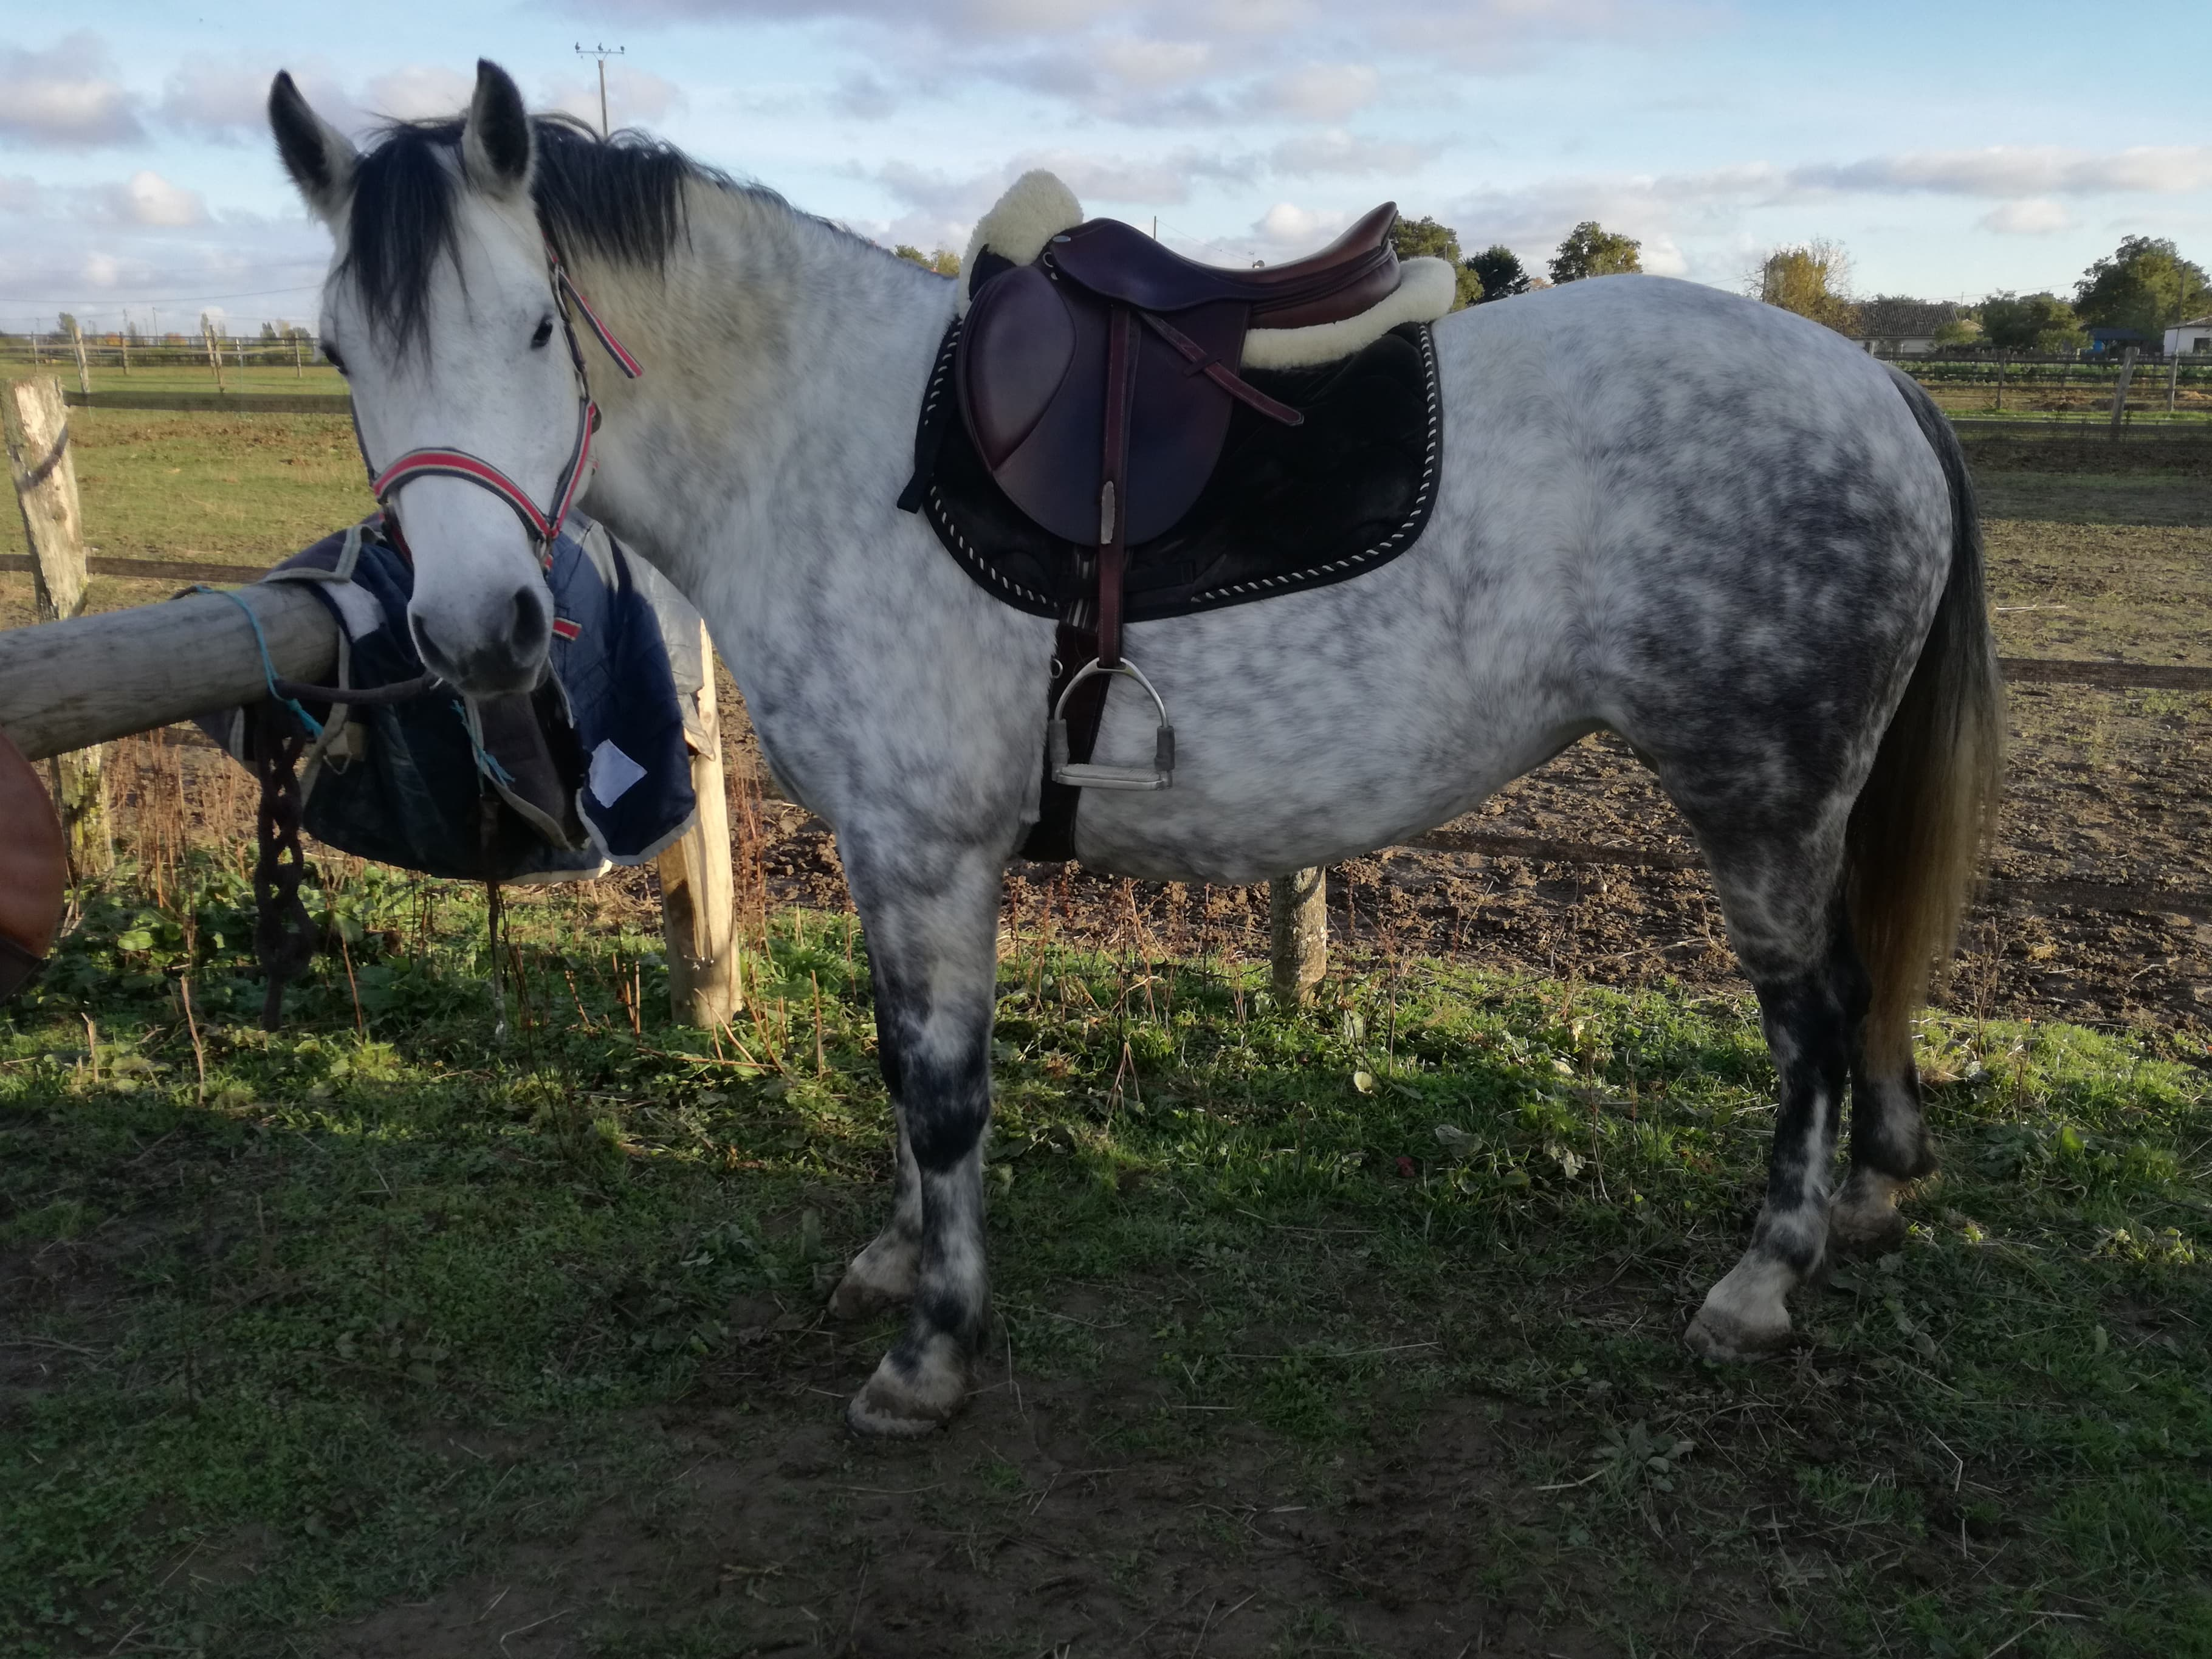
\includegraphics[width=0.5\textwidth]{./labwork/data/dada.jpg}
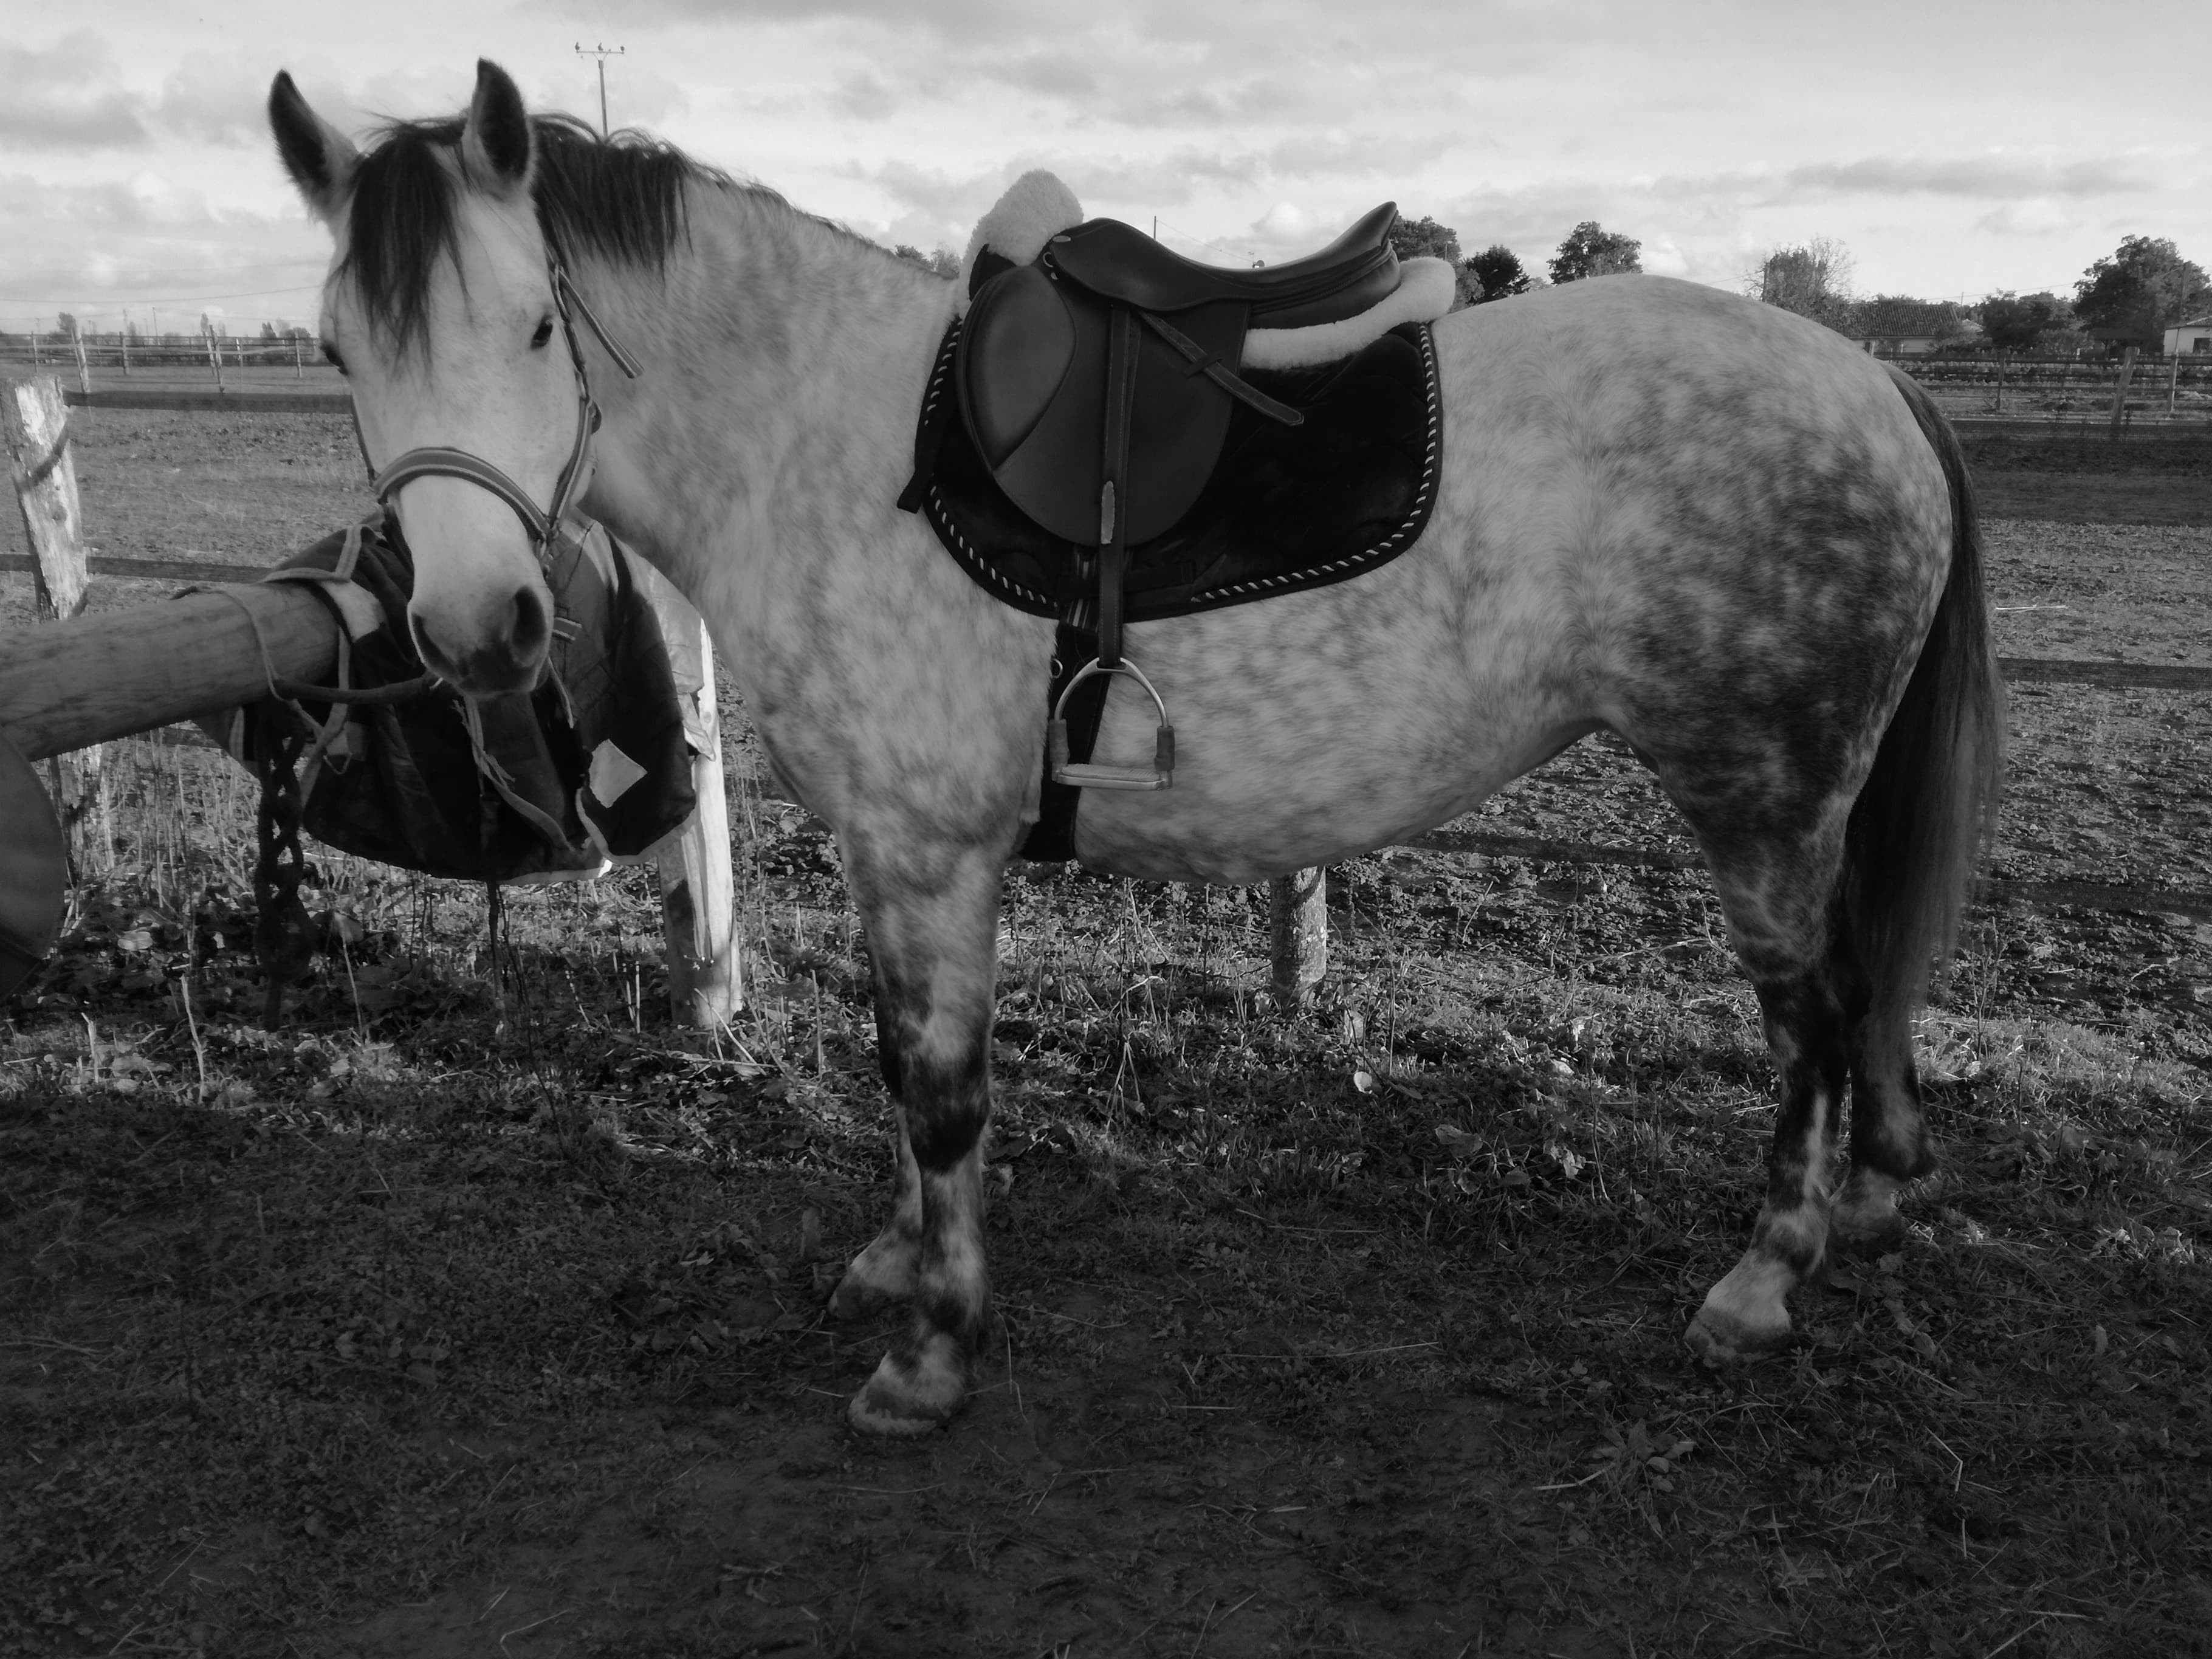
\includegraphics[width=0.5\textwidth]{./labwork7-gpu-out.jpg}
\caption{Result Image}
\end{figure}

\end{document}